\chapter{Implementation}
\label{cha:impl}
This chapter outlines the main stages in implementating the designed system in code.

% software environment to be mentioned in each section

The system to be developed, as initially described in Figure~\ref{fig:general}, is fairly representative of a Question-Answering(QA) system. QAs are data mining systems which use Information Retrieval(IR) and Information Extraction(IE) techniques to answer user queries. As such, this project was implemented in 3 stages, each corresponding to these subsystems in QA systems. The first of these was retrieving tweets, the IR phase of this project. Upon successful retrieval, information, the required features in this case, must be extracted and finally, these results must be displayed to the user in a simple, straightforward fashion. These stages will be further explored as follows:

\java
\section{Tweet Retrieval}
Without tweets, there is no work to be done, and so retrieving tweets can be regarded as the most important part of this project. The main objective of this stage is to retrieve as many relevant tweets from Twitter as possible. To do this, the system will interact with the set of public APIs Twitter provides in order to fulfill the requirements of each use case stated in Section~\ref{sec:uc}. The system is designed to use all of these to fulfill the requirements of each use case. This subsystem in the project is implemented in Java. This is because of its strong object oriented nature and platform independency. Of course, there are other options such as Python, however Java is a simple programming language with relatively straightforward multithreading capabilities.

\subsection{Streaming Twitter}
The Streaming API allows the system to fulfill the requirements of having a fully automated system that constantly monitors Twitter for software-related posts. 

The implementation at this stage utilises Twitter's filtering URL at \url{https://stream.twitter.com/1/statuses/filter.json} and passes it a set of dictionary terms and keywords to filter tweets by. This dictionary consists of a list of software, companies, operating systems and programming languages. The set of keywords contains words like \emph{release} or \emph{version}, which may be associated with software and are likely to be mentioned in software-related tweets. The full list of these dictionary items and keywords can be seen in Appendix~\ref{app:dictionary}.

This implementation could have been done using the \emph{Twitter4J}\footnote{\url{http://twitter4j.org/}} Java library for Twitter integration, however most of the functions appear unnecessary and excessive in the scope of this project. For this reason, the Twitter Streaming API integration was implemented from scratch.

Upon retrieving these filter terms from the database, the application formats this list into a string after which it creates three new Thread objects, a \emph{DatabaseThread} which will carry out all database operations, a \emph{StreamParseThread} which parses the stream of responses sent back from the Twitter server, and a \emph{ScannerThread}, which monitors the running state of the program, so as to allow a clean exit when the user wishes to quit. This scanner thread simply monitors the console input for users to type the exit command, upon which all connections are dropped and final parsing and database operations are carried out before closing the application. This high level control flow can be seen in Figure~\ref{fig:tweetir}.

On initialising these threads, the application attempts to set up a secure connection to Twitter using the HTTPS protocol. It uses the POST method to write the string of filter terms to the server in order to being receiving tweets. Once this connection is fully set up, Twitter will return JavaScript Object Notation(JSON) strings for each tweet, and so a JSON parser is set up using the Google-Gson Java library\cite{gson}. The aforementioned threads are then started as the actual streaming process now begins.

For every tweet returned by the API, the application adds this JSON response, as a \emph{JsonObject}, to a queue in the \emph{StreamParseThread} class, using the following simple method:
\begin{lstlisting}[caption=Adding tweets to a parse queue, label=lst:queue]
private final List<JsonObject> parseList = new ArrayList<JsonObject>();

public boolean addTask(final JsonObject object) {
    synchronized (parseList) {
        return parseList.add(object);
    } // synchronized
} // addTask(JsonObject)
\end{lstlisting}

The parser thread now assumes control of the processing to be done, while the main thread continues to add to this \emph{parseList} queue. The parser thread has the sole task of parsing the information in this JSON object into a more meaningful \emph{Tweet} object. This class' properties can be seen in Listing~\ref{lst:tweetuser}. To do this, the JSON object first needs to be checked if it represents a tweet delete entity, that is, a object containing the ``delete'' key signifying a user has deleted their tweet. In such a case, Twitter requests that applications honour the user's requests and delete this tweet. If otherwise the JSON object is actually a tweet, the program extracts the Twitter user's details to check their locale. In cases where this is not English, a \texttt{null} value is returned and the tweet is ignored. If this test passes, all the remaining properties described in the \emph{Tweet} and \emph{User} classes are extracted and returned as a single Tweet object.

This Tweet object is encapsulated in an \emph{InsertKeywordTask} object. This class is an implementation of the \emph{DatabaseTask} interface, which is used to perform the different database operations when used in conjunction with the different \emph{DatabaseConnector} classes. The hierarchy of these classes can be seen in Figures~\ref{fig:dbtask} and \ref{fig:dbcon} respectively. To further clarify, the \emph{DatabaseThread} constructor takes a \emph{DatabaseConnector} object as an argument. This allows for a more extensible system as different types of database management systems can be used with the application. It must be noted that in the current implementation, the \emph{DatabaseThread} class has been implemented at a similarly high level of abstraction, and as such an \emph{SQLThread} extends this class for use with a MySQL database. The \emph{SQLThread} initialises with a \emph{TweetSQLConnector} object, as it only operates in classes related to tweet retrieval. The DatabaseThread class maintains its own queue of \emph{DatabaseTask} objects as the parser thread, previously seen in Listing~\ref{lst:queue}.

\begin{figure}[t]
\begin{center}
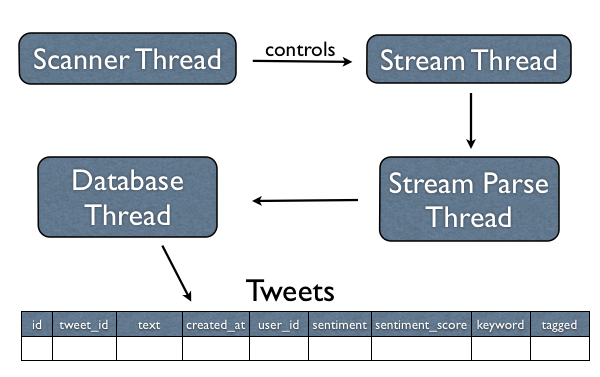
\includegraphics[width=12cm]{tweetir}
\end{center}
\caption{Control flow for tweet retrieval subsystem}
\label{fig:tweetir}
\end{figure}

\begin{lstlisting}[caption=Tweet and User class properties, label=lst:tweetuser]
public class Tweet {
    private final long tweetId;
    private final String tweet;
    private final String createdAt;
    private final User user;
    private String keyword = null; // Only used when filtering
    ...
} // class Tweet

public final class User {
    private final long id;
    private final String username;
    ...
} // class User 
\end{lstlisting}

\begin{figure}[h]
\begin{center}
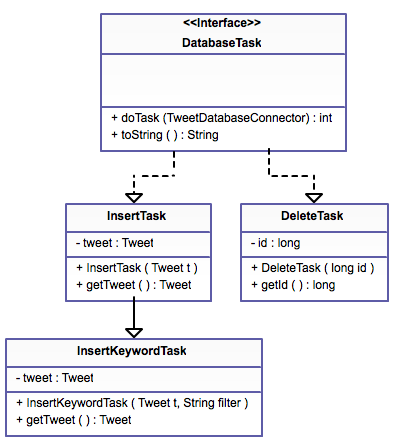
\includegraphics[width=7cm]{dbtask}
\end{center}
\caption{DatabaseTask class diagram}
\label{fig:dbtask}
\end{figure}

\begin{figure}[h]
\begin{center}
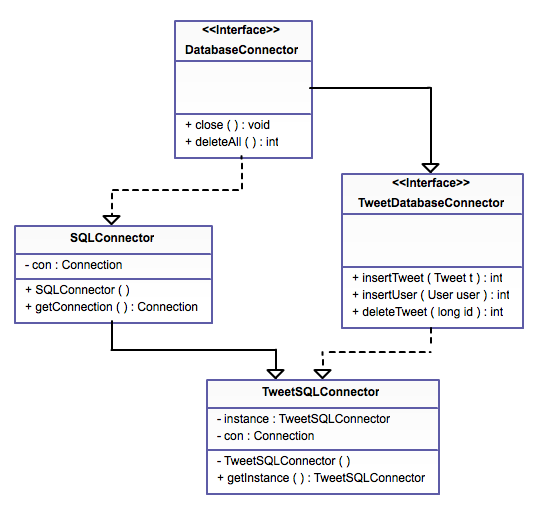
\includegraphics[width=9cm]{dbcon}
\end{center}
\caption{DatabaseConnector class diagram}
\label{fig:dbcon}
\end{figure}

Class design aside, once this \emph{InsertKeywordTask} object has been created, it is added to the queue in the \emph{DatabaseThread}. The respective implementations of the \emph{doTask()} method in each of the DatabaseTask classes will be performed as this queue is emptied. In the case of InsertKeywordTask, this is simply \texttt{db.insertTweet(t)}, where \texttt{db} is the TweetDatabaseConnector passed to it in the \texttt{doTask()} method, and \texttt{t} is the Tweet object it was initialised with.

This process is completed when the \emph{TweetDatabaseConnector} inserts the tweet into the database, in the current implementation using Java Database Connectivity(JDBC) to manipulate the MySQL server.

\subsection{Searching Twitter}
The Search API will now be used to handle the alternative use case of the designed system. With the Search API not operating in real time, the realisation of this use case can afford to be a much simpler system. The levels of multithreading displayed in streaming Twitter will not be required, as interaction with the API is more of a serial communication as can be seen in Figure~\ref{fig:ucsearch}.

\begin{figure}[h]
\begin{center}
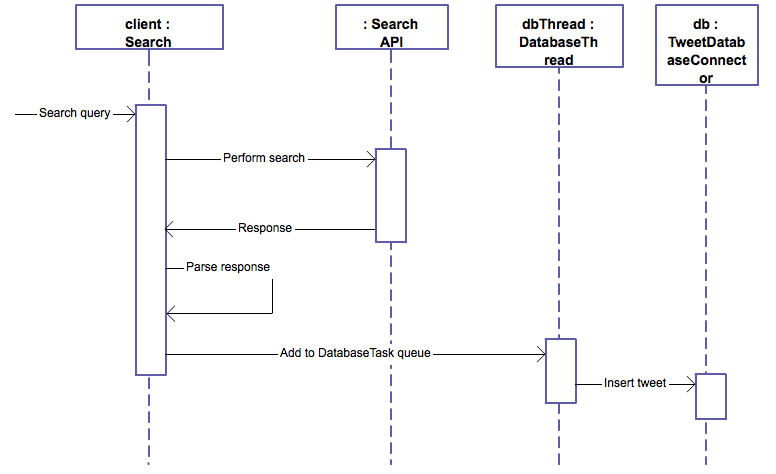
\includegraphics[width=13cm]{ucsearch}
\end{center}
\caption{Searching Twitter sequence diagram}
\label{fig:ucsearch}
\end{figure}

The implementation of the Twitter search use case utilises the Twitter Search API URL at \url{http://search.twitter.com/search.json}. The API also offers eXtensible Markup Language(XML) format responses, however, working with JSON allows consistency within the system. As with the implementation of the Twitter stream use case, the application begins with the initialision of a \emph{DatabaseThread} and is initially given a single keyword which will be searched for. This keyword is chosen by the end user. A simple HTTP GET request is then made to the above URL and Twitter then returns up to 1500 tweets from the last seven days corresponding to the search term.

The Search API returns a different JSON response to that of the Streaming API. Each JSON string contains an \texttt{iso\_language\_code}, and this will be used to filter tweets by language. Once the desired information has been extracted, i.e. the properties of the \emph{Tweet} class, the remaining operations are carried out just as they are in the realisation of the Twitter streaming use case, that is, the tweet is encapsulated in an \emph{InsertKeywordTask} object and this is added to a queue in the \emph{DatabaseThread} for the insert task to be carried out.

% SHOW KEYWORDS + DICTIONARY IN APPENDIX
% SHOW JSON RESPONSE IN APPENDIX


\python
\section{Feature Extraction}
Once tweets have been retrieved from Twitter and stored in the MySQL database, they are now available for feature extaction, which can be regarded as the core stage in implementing the system. This subsystem involves using NLP techniques to extract the information shown in Table~\ref{features} from each tweet. This subsystem is implemented in Python 2.7 due to the raw power it possesses and also due to the decision to use the Natural Language ToolKit(NLTK)\cite{NLTK}. NLTK is an active, well documented Python toolkit project. Alternatives to NLTK include GATE\footnote{\url{http://gate.ac.uk/}} and Minor Third\footnote{\url{http://sourceforge.net/apps/trac/minorthird/wiki}}. GATE is equally well documented, however it appears to be a bulky library, and many of its features are not required in the scope of this project. Minor Third on the other hand, is not as well documented, at the time of development at least, and as such would be more difficult to integrate. These alternatives are also Java implementations and it was felt that Python's speed and text manipulation would allow for a better implementation of the system.

There are many steps involved in implementing the feature extraction. These are explored in order of execution.

\subsection{Sentiment Analysis}
Sentiment analysis was recognised as one of the key features to be extracted from the initial design stages. It has been implemented using the Twitter Sentiment Bulk Classification Service API. This was chosen ahead of others such as AlchemyAPI\cite{alchemyapi} and the CLiPS Pattern modules. AlchemyAPI results were accurate, however with the massive number of tweets being streamed from the service it was not deemed feasible to continuously make calls to a web service to analyse them for sentiment, as the service only analyses individual tweets. As well as this, there is a limit of 10,000 tweets per day and with the large numbers of tweets posted on Twitter on the daily basis, this was also an issue.

While Pattern is an offline system, it states 72\% accuracy for movie reviews\cite{pattern}, while the Twitter Sentiment API is optimised for tweets and boasts 83\% accuracy\cite{Go_Bhayani_Huang_2009}. As well as this, the bulk classification service allows mass analysis with requests consisting of up to 10,000 tweets.

The sentiment analysis of tweets is carried out before any of the other feature extraction work. As tweets have been retrieved and stored in the MySQL database, this part of the system selects 100 of the latest tweets, retrieving just the id and text, that have yet to be analysed and packs them into a JSON string object of the format:

\begin{verbatim}
{ "data": [ { "id": "1234", "text": "Google Chrome is awesome!" },
            { "id": "1235", "text": "Safari 5.0.2 is out now" },
            { "id": "1236", "text": "I really hate the new Firefox" } ] }
\end{verbatim}

This JSON string is then posted to the Twitter Sentiment API where classifications into the positive, negative and neutral classes are carried out by a Maximum Entropy classifier trained with tweets containing emoticons. The internal specifics of a Maximum Entropy classifier, however, is not in the scope of this project. % further reading? CITE? APPENDIX?

Currently only 100 tweets are analysed at a time due to time constraints when users wish to run the program in real time. By using a small number, the data needing to be transferred is minimal and allows for a more interactive user experience.

Using the previous example, the data is returned by the server in the following format, with a polarity field added to each analysed tweet with values 0, 2 and 4 corresponding to negative, neutral and positive respectively.
\begin{verbatim}
{ "data": [ 
  { "id": "1234", "text": "Google Chrome is awesome!", "polarity": 4},
  { "id": "1235", "text": "Safari 5.0.2 is out now", "polarity": 2 },
  { "id": "1236", "text": "I really hate the new Firefox", "polarity": 0 } 
] }
\end{verbatim}

Upon receipt of this response, the JSON formatted string is parsed and the corresponding record for the tweet previously stored in the MySQL database is updated with new values for sentiment score and the actual sentiment, using polarity and its semantic meaning respectively.

\subsection{URL Extraction}
Before extracting context and semantics from tweets, any URLs mentioned are found and removed. Assuming the tweet is software-related, these URLs are quite likely to be links to the software, or further reviews. This task is done using NLTK's \texttt{regexp\_tokenize()} function with \url{http://}\verb/[^ ]+/ passed as the regular expression that finds URLs. If the tweet is later found not to contain any software, these URLs are discarded. Potential issues with this implementation could be that a user may post a URL without the preceeding \url{http://} protocol prefix and these would not be found by this regular expression. However, Twitter automatically converts URLs to their \url{http://t.co/} domain and so this is resolved on the Twitter server side.
%\subsection{Version}? OR LEAVE TILL NGRAM

\subsection{Tokenisation}
After URLs have been extracted and removed from the source text, the tweet is tokenised to produce an array of all the terms in the tweet. The tokenisation process is also done using NLTK's \texttt{regexp\_tokenize()} function, passing it the regular expression - \verb/\w+([.,]\w+)*|\S+/. This expression returned superior results to alternation tokenisation functions provided by NLTK, such as \texttt{wordpunct\_tokenize()} as it was capable of finding numbers and currencies without splitting them. Using the above example,

\begin{quote}
I really hate the new Firefox
\end{quote}
this would be tokenised to the following:
\begin{quote}
[`I', `really', `hate', `the', `new', `Firefox']
\end{quote}

The following example shows a more complicated tokenisation process.
\begin{quote}
Norton Anti-Virus released for \$50 \#ripoff

\begin{math}\Rightarrow\end{math}
[`Norton', `Anti', `-Virus', `released', `for', `\$50', `\#ripoff']
\end{quote}

\subsection{Price Extraction}
Continuing on from this tokenisation of the original source text, the current subsystem attempts to find prices in the array of terms. This is done using Python's built-in regular expression module, \texttt{re}. A number of regular expressions are used to define patterns denoting numbers, currencies and quantifiers like `hundred' and `thousand'. As the form of prices vary, for example in the case of mobile apps you might find `£0.59', `59p' or even `59 pence', these combinations of tokens may be split across two tokens in the array returned from the tokenisation process. For this reason, it is necessary to iterate over all items in the list of tokens while remembering the previous one. This obviously means a less efficient system, however, it has produced the best results in such variable conditions.

\subsection{Part-of-speech (POS) Tagging}
The POS tagger used by this system is taken from the NLTK modules and uses the \texttt{pos\_tag()} function which takes a tokenised sentence as its only argument. Continuing from the first example, this process tags as follows: 
\begin{quote}
[`I', `really', `hate', `the', `new', `Firefox']

\begin{math}\Rightarrow\end{math}
[(`I', `PRP'), (`really', `RB'), (`hate', `JJ'), (`the', `DT'), (`new', `JJ'), (`Firefox', `NNP')]

\begin{center}
\begin{tabular}{ l | l }
  \hline                        
  PRP & Pronoun \\
  RB & Adverb \\
  JJ & Adjective \\
  DT & Determiner \\
  NNP & Proper Noun \\
  \hline  
\end{tabular}
\end{center}
\end{quote}

\subsection{N-Grams}
N-grams are sequences of n tokens from a given source text. The implementation of creating n-grams in this project is done using the \texttt{nltk.util.ngrams()} function. This process starts by creating a five-gram of the tweet tokens. This means a sequence of five tokens will be created from the array of tokens. The system utilises a five-gram sequence due to potentially long software names, basing this on the na\"{\i}ve assumption that these names will not exceed five words. This will allow for improved extraction of software names in the next stage. Using the Firefox tweet as a running example, the outcome of this five-gram modelling process can be seen below.

\begin{quote}
[`I', `really', `hate', `the', `new', `Firefox']

\begin{math}\Rightarrow\end{math}

[
 ( (`I', `PRP'), (`really', `RB'), (`hate', `JJ'), (`the', `DT'), (`new', `JJ') ),

 ( (`really', `RB'), (`hate', `JJ'), (`the', `DT'), (`new', `JJ'), (`Firefox', `NNP') )
]
\end{quote}

\subsection{Main Feature Extraction}
This tagging process consists of the core functions of the proposed system. Its purpose is to extract all the features that have yet to be extracted, that is, software names and versions, companies, programming languages and operating systems. It also attempts to find any prices that may previously have been missed, and also has the task of discovering software that is not already in the dictionary.

Having created a set of five-gram sequences from the tweet, the application may now iterate through each of these in an attempt to find any information that has not yet been found.

\begin{lstlisting}[caption=Example of some extracted features, label=lst:extr]
{
  `programming_language_id' : `317',
  `programming_language_name' : `python',
  `software_id' : `159',
  `software_name' : `moodle',
  `tweet' : `Best Affordable Drupal, Python, Moodle Hosting: 
             Top 3 Drupal, Python, Moodle Web Hosts http://t.co/0WHPTsns',
  `tweet_db_id' : `440094',
  `url' : `http://t.co/0WHPTsns'
}
\end{lstlisting}

\subsection{Software Verification}
The feature extraction subsystem may discover new software, and as such needs to verify these are actually pieces of software and not something else. To do this the program utilises the Microsoft Bing API which returns web search queries. As the main tagging process checks the dictionary for matching software names, and the tweet retrieval engine uses both the dictionary and a set of keywords, there will be some pieces of software mentioned in the tweets that are not in the dictionary. As a result, these will be flagged as possible software names, and then queried on the Microsoft Bing search engine with the keywords ``movie'', ``music'', and ``software game''. These keywords were selected on the basis that the initial search key terms retrieved many tweets referring to music and films.
\begin{verbatim}
function bing_search(bing, term){
    music = bing.search(term, music)
    movie = bing.search(term, movie)
    software = bing.search(term, software game)

    if size(software) greater than size(movie) and size(music)
        if references to software in title and description
            return True
    return False
}
\end{verbatim}
If the number of results for software associated with the searched term is greater than corresponding results for films and music, the results are checked for identifiers of software in their headings. Therefore if any of the results suggests the searched term is a piece of software, that is assumed true.

% BING.PY IN APPENDIX

\section{Storing the Extracted Information}
As the information being extracted is temporarily stored in a Python dictionary variable, it is essentially in the form of a JSON string. The database design for storing this information is also in the form of a NoSQL database. For this reason, a document-based database system seems to be the best approach. MongoDB\footnote{http://www.mongodb.org/} is a document-oriented NoSQL database, which stores JSON-style documents. By using MongoDB, it is easy to store the extracted information, as it is as straightforward as directly storing the string representation of this variable as a record in the database.

\section[Visualisation]{Visualisation/Graphical User Interface(GUI)}
The final stage of the project is to aggregate and present the results to the user in a GUI.
Aggregating the results is the process of bringing together all the different data sources for data on a single output entity such as a piece of software. This aggregated data can then be used easily by the GUI to display understandable information to the user.
The GUI of choice is a web application as opposed to a desktop application, as it allows for a more centralised system that users can easily connect to. It is also a more scalable solution as updates would not need to be pushed out to all users.

\subsection{Aggregation}

% SHOW MONGO FUNCTIONS
\subsection{Web Application}
The web application available to users is a Python application running the CherryPy web framework.
